\documentclass[11pt, oneside,table]{article}   	% use "amsart" instead of "article" for AMSLaTeX format
%\usepackage{geometry}                		% See geometry.pdf to learn the layout options. There are lots.
\usepackage[margin=.9in]{geometry}
\geometry{letterpaper}                   		% ... or a4paper or a5paper or ... 
%\geometry{landscape}                		% Activate for for rotated page geometry
\usepackage[parfill]{parskip}    		% Activate to begin paragraphs with an empty line rather than an indent
\usepackage{graphicx}				% Use pdf, png, jpg, or eps� with pdflatex; use eps in DVI mode
\usepackage{moreverb}						% TeX will automatically convert eps --> pdf in pdflatex		
\usepackage{amssymb}
\usepackage{mathtools}
\usepackage[framed,numbered,]{mcode}
\usepackage{listings}
\usepackage{xcolor}
\usepackage{amsmath}
\lstset { %
    backgroundcolor=\color{black!7}, % set backgroundcolor
    basicstyle=\footnotesize,% basic font setting
}

\newcommand{\bigo}{$\mathcal{O}$}

\title{MATH 6644\\Project 1}
\author{Stephan Boettcher}
%\date{}                                           % Activate to display a given date or no date

\begin{document}
\maketitle
\section*{Part 1}

{\it Discretize the following differential equation:

$$\begin{cases} -u'' =2x-\frac{1}{2}& \ \ x\in [0,1] \\ u(0)=1, & u(1)=-1 \end{cases}
$$
by centered difference scheme with n interior mesh points. Solve the resulting linear system by Conjugate Gradient (CG), Preconditioned CG with Sine transform to construct the preconditioner.}

The one-dimensional equation given above can be solved with numeral method analysis or directly as a function of x. The solved equation then can be used to check the validity of the numerical methods. When solved directly, the equation becomes:
$$u(x) = -0.333333 x^3+0.25 x^2-1.91667 x+1
$$


The discretized one-dimensional equation above was solved by the central difference scheme with $n$ interior points. The resulting problem is then an $(n+2)\times (n+2)$ matrix, A, and $(n+2)\times 1$ vectors, x and b. The problem was solved using both the Conjugate Gradient (CG) method and the Preconditioned CG method with a Sine transform preconditioner, $S$. The $S$ matrix was defined as:

$$[S]_{j,k}=\sqrt{\frac{2}{n+1}}sin\Big(\frac{\pi jk}{n+1}\Big)
$$

The A matrix formed from the discretized equation forms a tridiagonal matrix, with elements directly on the primary diagonal as well as elements one diagonal above and below the primary diagonal. This sparse matrix was then run with the Conjugate Gradient(CG) method. The CG method is one of the most prominent iterative methods for solving sparse matrices as it converges much more quickly than other iterative methods such as steepest descent. The Conjugate Gradient iterates in such a way that each new residual is orthogonal to all the previous residuals and search directions. Each new search direction is constructed is A-orthogonal to all the previous residuals and search directions, thus using the Krylov subspace to iterate more efficiently. The CG method was run with $n$ interior points from 256 to 16384. As the values of $n$ increased, the time necessary to complete the iteration increased proportionally. The final results of the CG method can be found in Figure \ref{p1}.  Figure \ref{final} shows the CG method approaching After the CG method completed, the $S$ matrix, used in the PCG method, was formed. 

%\begin{figure}[!h]
%\begin{center}
%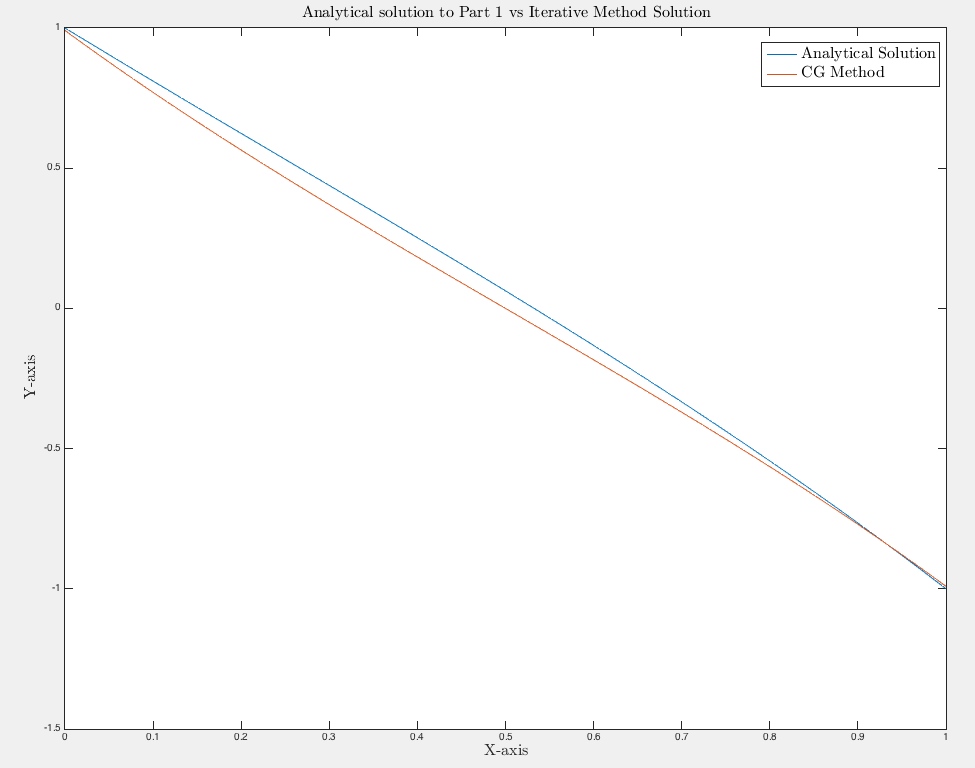
\includegraphics[width=130mm]{p1s.png}
%\caption{Convergence of the CG method.}
%\label{final}
%\end{center}
%\end{figure}

The $S$ matrix was formed in two different ways to determine the most efficient method. The first method was using Matlab's vector math and \mcode{parfor} to form the matrix in parallel. This was achieved with the following code:

\begin{lstlisting}
k=1:runs(a); %generates a vector from 1 to the length of n. 
%runs contains the list of n values and a is the current iteration.
parfor j=1:runs(a)  %Parallel for loop in matlab
        S(j,k)=sqrt(2/(n+1))*sin((pi*j*k)/(n+1)); %form an entire column of values
end
\end{lstlisting}

This code was run with 4 workers in parallel, allowing for a theoretical 4x improvement over the serial code. Figure \ref{parfor} shows the runtime for the parallel code vs serial code.  As is common with parallel code, for small values of $n$, the serial code outperforms the parallel. However, for larger $n$ values, the 4x speedup is achieved. The $S$ matrix then was formed using Matlab's Discrete Sine Transform(DST) command, \mcode{dst(x)}. Figure \ref{parfor} shows the runtime for the built in DST command which proved to be slower than the parallel code. Thus for the remainder of this portion of the project, the parallel code was used. 

\begin{figure}[htbp]
\begin{center}
\begin{tabular}{ | c|c|c| c|}
\hline
  n & Serial (sec) & Parallel For(sec) & DST (sec)\ \\\hline
  258 &0.0194 & 0.0494& 0.5190 \\\hline
  514 &0.0111 & 0.0564 & 0.0196\\\hline
  1026 &0.0423 & 0.0771 & 0.0706\\\hline
  2050 &0.1704 & 0.1439 & 0.2003 \\\hline
  4098 &0.5087 & 0.4694 &1.1024 \\\hline
  8194 &8.1068 & 1.9299 & 3.9583\\\hline
  16386 &37.3268 & 7.9876 & 29.3784\\\hline
  % Design2 &300 & 380 & 370 & 34 & 40& 400& 100& 50& 100& 100 \\\hline
%  Design3 &300 & 600 & 580 & 40 & 50& 550& 100& 150& 200& 250 \\\hline

\end{tabular}
\caption{Runtime for generating the $S$ }
\label{parfor}
\end{center}
\end{figure}



The $S$ matrix acted as a preconditioner to the tridiagonal $A$ matrix. A preconditioned is used to make a problem that is difficult to solve, simpler. The preconditioner is customized and tailored to the problem at hand. For this problem, preconditioning the $A$ matrix by $SAS^T$ results in a diagonal matrix. To achieve extremely fast convergence rates, the preconditioner matrix was split. After preconditioning $A$ with the $S$ matrix, the  inverse, $(SAS^{T})^{-1}$, was calculated and passed to the PCG method. As a result, the PCG method was able to achieve extremely fast convergence rates. While this method does require two matrix-matrix multiplications to setup the preconditioned $A$ matrix, the resulting diagonal matrix was extremely easy to solve. The inverse of the diagonal matrix, $(SAS^{T})^{-1}$, can be calculated in  \bigo(n) time, as the inverse of a diagonal matrix is the inverse of each element on the diagonal. With the chosen preconditioner, each run of the PCG was able to converge in 1 iteration. 


\begin{figure}[htbp]
\begin{center}
\begin{tabular}{ |c|c|c| c|c|}
\hline
  n & CG iterations & CG runtime (sec) & PCG iterations & PCG runtime (sec)\ \\\hline
258 & 129 & 0.023895 & 1 & 0.294494 \\\hline
514 & 257 & 0.014975 & 1 & 0.023645 \\\hline
1026 & 513 & 0.193338 & 1 & 0.111805 \\\hline
2050 & 1025 & 2.468402 & 1 & 0.809114 \\\hline
4098 & 2049 & 18.554962 & 1 & 5.579513 \\\hline
8194 & 4097 & 145.323975 & 1 & 40.182528 \\\hline
16386 & 8193 & 1144.595261 & 1 & 326.499772 \\\hline
  % Design2 &300 & 380 & 370 & 34 & 40& 400& 100& 50& 100& 100 \\\hline
%  Design3 &300 & 600 & 580 & 40 & 50& 550& 100& 150& 200& 250 \\\hline

\end{tabular}
\caption{Runtimes and iteration counts for the CG and PCG methods }
\label{p1}
\end{center}
\end{figure}

As can be seen in Figure \ref{p1}, the PCG method is able to converge in one iteration and in much less time than the CG method. When recording the timing for the PCG method, the time required to form the $S$ matrix was not accounted for, but can be found in Figure \ref{parfor}. The recorded time for the PCG method did account for the two costly matrix multiplication operations, which were undoubtedly the source of much of the runtime. Regardless, the results are impressively conclusive. The PCG method is significantly faster than the regular CG method for this problem. The runtimes for both methods actually decrease for the $n=512$ interior mesh point case ($n=514$ total points). This is actually due to bandwidth/latency optimizations that are occurring at the processor/memory cache level. As n increases, the number of CG iterations also roughly doubles. However, for both the CG and the PCG method, the time to complete the method increase by a factor of 8. The primary driver of this increase is the matrix multiplication that occurs in each method. 







\section*{Part 2}




{\it Perform the CG and PCG for Toeplitz systems using both Strang's and Chan's circulant matrices as the preconditioners..} \newline
Beginning with the dense A matrix of: $
A = \begin{bmatrix}
1& 2& 1          \\[0.3em]
4& 9           & 2 \\[0.3em]
     7           & 20 &2
     \end{bmatrix}
  $ , we generate the G matrix by first constructing the N and M matrices. The M matrix is defined as the diagonal elements of A and the N matrix is defined as: N=M-A, or the off diagonal elements multiplied by -1. The G matrix is then constructed by $G=M^-1*N$, which creates the following matrix:
$
G = \begin{bmatrix}
0 & -2& -1          \\[0.3em]
       -\frac{4}{9} & 0           & -\frac{2}{9} \\[0.3em]
       \frac{7}{2}           & -10& 0
     \end{bmatrix}
  $ .  The spectral radius of the G matrix is 2.9413. This spectral radius makes for an unstable iteration matrix that will most likely result in the iterative method going to infinity, rather than converging on a value. An iteration for this matrix is defined as: 
  $$ \vec{x}_{k+1}=G\vec{x}_k+\vec{c}
  $$

\section*{Question 5}
{\it Discreteize the following differential equation:
$$\begin{cases} -u'' +4u = & x\in [0,1] \\ u(0)=-1, & u(1)=2 \end{cases}
$$

by the central difference scheme. Write your linear system of equations (you must give the matrix A and $\vec{b}$). Solve the system by using classical iteration such as Jacobi, Gauss-Seidel and SOR with n = 1000. Test you relaxation parameter in SOR for several values and decide which one is better. You need to discuss your results.}\newline

The above differential equation can be solved analytically to generate a truth curve, against which the numerical methods can be compared. The solution for this particular ODE is:
$$u(x)=\frac{e^{-2x}(e^{4x}+2e^{4x+2}-2e^2-e^4)}{e^4-1}
$$

To solve this equation numerically, the equation must first be discretized via the central difference theorem. The first step is to discretize the term $-u''$:
$$u''=\frac{d^2u}{dx^2}=\frac{1}{h}\Bigg(\frac{u(x+h)-u(x)}{h}-\frac{u(x)-u(x-h)}{h}\Bigg) = \frac{1}{h^2}\bigg(u(x+h)-2u(x)+u(x-h)\bigg)
$$

This gives the final form of the differential equation, with the same boundary conditions, of:
$$0=-\frac{1}{h^2}\bigg(u(x+h)-2u(x)+u(x-h)\bigg)+4u(x)
$$
Realizing that $h=x_i-x_{i-1}$, this can be simplified and rewritten as:
$$0=u_{i+1}-2u_i+u_{i-1}-4h^2u_i
$$

This form of the equation can be used to generate the A and $\vec{b}$ variables, where $A\vec{u}=\vec{b}$:

{\begin{center}
$A= \begin{bmatrix}
-2-4h^2 & 1 &0 &0 &0&\dots&0          \\[0.3em]
1 &-2-4h^2 & 1 &0 &0&\dots&0     \\[0.3em]
0 &1 &-2-4h^2 & 1 &0 &\dots&0 \\[0.3em]
&&\ddots &\ddots &\ddots \\[0.3em]
0&\dots&\dots&\dots&\dots&1&-2-4h^2 
     \end{bmatrix}
  $  ,  $\vec{u} = \begin{bmatrix}
u_1          \\[0.3em]
u_2\\[0.3em]
\vdots \\[0.3em]
u_{n-2}\\[0.3em]
u_{n-1}
     \end{bmatrix}
  $  ,  $\vec{b}= \begin{bmatrix}
1          \\[0.3em]
0 \\[0.3em]
\vdots\\[0.3em]
0\\[0.3em]
-2
     \end{bmatrix}
  $ 
  \end{center}
where $h=\frac{1}{n}$. This discretized ODE was then solved using the Gauss-Jacobi , Gauss-Seidel, and SOR with $n=1000$. 

The A matrix as well as the b and u vectors were created with the following code:
\lstinputlisting{SetupProb1.m}
The first algorithm tested was the Gauss-Jacobi method. This is the simplest algorithm to implement and has a simple iteration. The G-J method is computed by the equation: 
$$x_i^{(k+1)}=\frac{1}{a_{ii}}\bigg(b_i+\sum\limits_{\substack{j=1\\ j\ne i}}^n a_{ij}x_j^{(k)}\bigg) \ \ \ \ \ \ \ \ i=1:n
$$
The G-J algorithm can quickly be implemented in just a few lines in Matlab, using Matlab's vector notation. The implementation used for this problem is shown below.
\lstinputlisting{Jacobi.m}
The G-J method was run with a number of different convergence criteria to demonstrate the convergence properties of this method. Figure \ref{gj} shows these convergence values. The convergence criteria is defined as $|\vec{x}^{\ (k+1)}-\vec{x}^{\ (k)}|$. When the method is no longer making any significant changes to the $\vec{x}$ values, it has been deemed converged. This is used throughout this homework question as a metric for performance. 


\begin{thebibliography}{9}
\bibitem{Painless}
 Jonathan Richard Shewchuk,
  \emph{An Introduction to the Conjugate Gradient Method Without the Agonizing Pain}.
  Carnegie Mellon University
  1994.

\end{thebibliography}



%\begin{figure}[htbp]
%\begin{center}
%\begin{tabular}{ | l | c|c| c| c | c | c| c| c| c  | c | }
%\hline
%  &A & B & C &D &E&F&G&H&I&J\ \\\hline
%  Design1 &240 & 350 & 305 & 30 & 35& 400& 90& 0& 30& 300 \\\hline
%% Design2 &300 & 380 & 370 & 34 & 40& 400& 100& 50& 100& 100 \\\hline
%%  Design3 &300 & 600 & 580 & 40 & 50& 550& 100& 150& 200& 250 \\\hline
%
%\end{tabular}
%\caption{Design 1 Parameters}
%\end{center}
%\end{figure}
%
%The isometric view of this design can be seen in Figure \ref{d1i}. The large cylinder was plotted using multiple instances of the \mcode{surf} command on two cylinders. Figure \ref{d1y} and Figure \ref{d1z} show the printer design in the X-Y and X-Z plains, respectively.
%
%\begin{figure}[htbp]
%\begin{center}
%\includegraphics[width=160mm]{d1iso.png}
%\caption{An isometric view of Design 1}
%\label{d1i}
%\end{center}
%\end{figure}



\end{document}  